\documentclass[a4paper, 12pt]{article}

\renewcommand{\familydefault}{\sfdefault}

\usepackage[english]{babel}
\usepackage{amsmath}
\usepackage{amssymb}
\usepackage{parskip}
\usepackage{graphicx}
\graphicspath{ {./images/} }
\usepackage{capt-of}

\begin{document}
\title{\Large{\textbf{Machine Learning Algebra}}}
\author{By Matthieu Lagarde}
\date{April 9, 2022}

\maketitle

\setcounter{page}{2}

\newpage
\section{Multivariate linear regression}
\subsection{Notations}

Let $m$ be the number of examples or observations in our training set. Let $n$ be the number of features or explanatory variables observed for each example of the training set. Let $x_j^{(i)}$ be the value of feature $j$ for example $i$. Let $y^{(i)}$ be the output value for example $i$.

\begin{equation}
y = \begin{pmatrix}  y^{(1)} \\ y^{(2)} \\ ... \\ y^{(m)} \end{pmatrix} \in \mathbb{R}^{m} 
\end{equation}

\noindent
$y$ is called the output vector. It contains the output values of the training set.

\begin{equation}
X = \begin{pmatrix} 1 & x_1^{(1)} & x_2^{(1)} & ... & x_n^{(1)} \\  1 & x_1^{(2)} & x_2^{(2)} & ... & x_n^{(2)} \\ ... & ... & ... & ... \\ 1 & x_1^{(m)} & x_2^{(m)} & ... & x_n^{(m)} \end{pmatrix} \in \mathbb{R}^{m\times(n+1)} 
\end{equation}

\noindent
$X$ is called the data matrix. If we ignore the first column of $1$, each row of matrix $X$ is one example of the training set and each column of the matrix $X$ is the values observed for one feature in the training set.

\begin{equation}
\theta = \begin{pmatrix}  \theta_0 \\ \theta_1 \\ ... \\ \theta_n \end{pmatrix} \in \mathbb{R}^{(n+1)} 
\end{equation}

$\theta$ is the vector of parameters.

\subsection{Hypothesis}

We assume that there is a linear relationship between the features and the output. Note that the relationship is linear in $\theta$ but the features themselves can be non linear transformations of the initial features such as quadratic terms or interaction terms.

\noindent
The unvectorized form of the hypothesis for a given example $i$ is:

\begin{equation}
h_{\theta}(x^{(i)}) = \sum_{j=0}^{n} \theta_j * x_j^{(i)} \in \mathbb{R} \; with \;  x_0^{(i)}=1
\end{equation}

\noindent
The vectorized form of the hypothesis can be written as follows:

\begin{equation}
h_{\theta}(X) = X\theta \in \mathbb{R}^{m} 
\end{equation}

\noindent
For a single example, we can also write the vectorized form of the hypothesis:

\begin{align*} 
& x^{(i)} = \begin{pmatrix} 1 \\ x_1^{(i)} \\ ... \\ x_n^{(i)} \end{pmatrix}  \in \mathbb{R}^{(n+1)}  \\
& \\
& h_{\theta}(x^{(i)})  = x^{(i)^{\top}}\theta \in \mathbb{R}
\end{align*}

\subsection{Cost function}

\noindent
The unvectorized form of the cost function is:

\begin{align*}
& J(\theta) = \frac{1}{2m} * \sum_{i=1}^{m} (h_{\theta}(x^{(i)}) - y^{(i)})^{2} \in \mathbb{R} \\
& where \; x^{(i)} \in \mathbb{R}^{(n+1)} \; and \\
& where \; y^{(i)} \in \mathbb{R}
\end{align*}

\noindent
The vectorized form of the cost function is:

\begin{equation}
J(\theta) = \frac{1}{2m} * (X\theta - y)^{\top}(X\theta - y) \in \mathbb{R}
\end{equation}

\subsection{Normal equation}

$J(\theta)$ is convex so any local minimum is  a global minimum. We thus know that $\theta^{*}$ obeys the following equation:

\begin{align*}
\nabla J(\theta^{*}) = 0_{(n+1)}
\end{align*}

Let recall a property of matrix differentiation. Let $\alpha$ be a scalar equal to $y^{\top}x$ where $y$ and $x$ be two column vectors of $\mathbb{R}^m$ that are respectively a function of another column vector $z$ of $\mathbb{R}^n$. We have:

\begin{align*}
& \alpha = y^{\top}x \\
& \\
& \frac{\partial \alpha}{\partial z}= {\frac{\partial y}{\partial z}}^{\top}x + {\frac{\partial x}{\partial z}}^{\top}y \in \mathbb{R}^n
\end{align*}

Using this property, we have:

\begin{align*}
& 1/2m*2*{\frac{\partial (X\theta^* - y)}{\partial \theta}}^{\top}(X\theta^* - y) = 0_{(n+1)} \\
& \iff 1/m*X^{\top}(X\theta^* - y) = 0_{(n+1)} \\
& \iff X^{\top}X\theta^* - X^{\top}y = 0_{(n+1)} \\
& \boxed{\iff \theta^* = {(X^{\top}X)}^{-1}X^{\top}y \in \mathbb{R}^{(n+1)}}
\end{align*}

\subsection{Gradient descent}

If necessary, here is the vectorized implementation of gradient descent. Denoting $\alpha$ the learning rate:

\begin{equation}
\theta := \theta - \frac{\alpha}{m} * X^{\top}(X\theta- y) \in \mathbb{R}^{(n+1)}
\end{equation}

\subsection{Regularized cost function}

Denoting $\lambda$  the regularization parameter, the unvectorized form of the cost function can be written as:

\begin{align*}
& J(\theta) = \frac{1}{2m} * \sum_{i=1}^{m} (h_{\theta}(x^{(i)}) - y^{(i)})^{2} + \frac{\lambda}{2m}*\sum_{j=1}^{n} \theta_j^{2}  \in \mathbb{R} \\
& where \; x^{(i)} \in \mathbb{R}^{(n+1)} \; and \\
& where \; y^{(i)} \in \mathbb{R}
\end{align*}

Be careful, in the regularization part of the expression (the second sum), the $j$ index goes from $1$ to $n$ and NOT from $0$ to $n$. Indeed, by convention, we do not regularize $\theta_0$.

The vectorized form of the regularized cost function is thus:

\begin{align*}
& J(\theta) =  \frac{1}{2m} * (X\theta - y)^{\top}(X\theta - y) + \frac{\lambda}{2m}*\theta_{r}^{\top}\theta_{r} \\
& where \; \theta_{r} =  \begin{pmatrix}  \theta_1 \\ ... \\ \theta_n \end{pmatrix} \in \mathbb{R}^{n} 
\end{align*}

\subsection{Regularized normal equation}

The vectorized form of the regularized normal equation is:

\begin{align*}
& \theta^* = {(X^{\top}X + \lambda*M)}^{-1}X^{\top}y \in \mathbb{R}^{(n+1)} \\
& where \; M = \begin{pmatrix}0 & 0 & 0 & ... & 0 \\ 0 & 1 & 0 & ... & 0 \\ ... & ... & ... & ... & ... \\ 0 & 0 & ... & 1 & 0 \\ 0 & 0 & ... & 0 & 1\end{pmatrix} \in \mathbb{R}^{(n+1)\times(n+1)}
\end{align*}

\subsection{Regularized gradient descent}

Let compute the gradient of $J(\theta)$ when it is regularized. There are two cases, one for the partial derivative with respect to $\theta_0$ and one for the partial derivatives with respect to $\theta_j$:

\begin{align*}
& \frac{\partial J(\theta)}{\partial \theta_0} = {\left[ \frac{1}{m}*X^{\top}(X\theta-y) \right]}_{1} \; i.e. \; 1st \; element \; of \; previous \; gradient \\
& \\
& \frac{\partial J(\theta)}{\partial \theta_j} = {\left[ \frac{1}{m}*X^{\top}(X\theta-y) + \frac{\lambda}{m} * \theta \right]}_{j+1} \; for \; j \in \{1, 2, ..., n\} 
\end{align*}

\section{Logistic regression}

\subsection{Sigmoid function}

Let introduce the sigmoid function:

\begin{equation}
g \; : \; x \in \mathbb{R} \longrightarrow  \frac{1}{1+e^{-x}} \in \left] 0, 1 \right[
\end{equation}

The interesting properties of the sigmoid function are:
\begin{itemize}
\item It is defined over $\mathbb{R}$.
\item It is increasing. 
\item $g(0) = \frac{1}{2}$.
\item It is converging to 0 in $-\infty$ and to 1 in $+\infty$.
\item It is convex over $\left] -\infty, 0 \right]$ and concave over $\left[ 0, +\infty \right[$.
\item It means that (0, 0.5) is an inflection point of $g$.
\item $g(-4) = 0.02 $ and $g(4) = 0.98 $
\end{itemize}

\begin{center}
  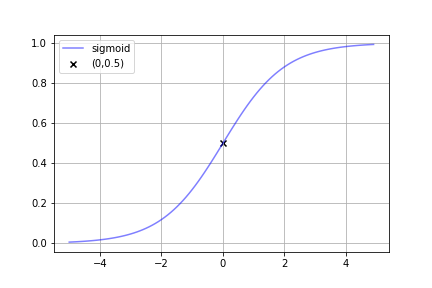
\includegraphics[scale=0.7]{sigmoid}
  \captionof{figure}{Graph of the sigmoid function}
  \label{fig:sigmoid}
\end{center}

\subsection{Hypothesis}

\noindent
The unvectorized form of the hypothesis for a given example $i$ is:

\begin{align*}
& h_{\theta}(x^{(i)}) = g \left( \sum_{j=0}^{n} \theta_j * x_j^{(i)}  \right) \in \left]0, 1\right[  \\
& \\
& where \; g \; is \; the \; sigmoid \; function.
\end{align*}

The hypothesis can be interpreted as the probability that a new observation belongs to the positive class i.e. that $y=1$ given the value of its features i.e. given $x$, parameterized by $\theta$. In other words:

\begin{equation}
h_{\theta}(x) = P\left(y=1|x;\theta \right)
\end{equation}

We then introduce the following decision rule:

\begin{equation}
y = 
\begin{cases}
1 & \text{if } h_{\theta}(x) \geq 0.5 \\
0 & \text{if } h_{\theta}(x) < 0.5
\end{cases}
\end{equation}

\end{document}